\chapter{Electronic Excited States}

\begin{quote}
  "The XXIst century might be very well the century of light. Understanding and controlling photoexcited systems will be crucial for future research in many branches of optics and photonics."
  \begin{flushright}
    \small{--- \textit{L. González, D. Escudero, L. Serrano-Andrés (2011) [Gon2011] }}
  \end{flushright}
\end{quote}


% Gon2011 https://chemistry-europe.onlinelibrary.wiley.com/doi/10.1002/cphc.201100200

\section{Nature of Excited States}

The potential energy landscape of electronic excited states is complex and governed by various absorption and decay mechanisms. Excitations are generally grouped into three categories:
\begin{enumerate}
\item \emph{Valence excitations}, where valence electrons are excited into (local) higher lying unoccupied orbitals above the Fermi level
\item \emph{Rydberg excitations}, where electrons are excited into very diffuse orbitals around the molecule
\item \emph{Charge transfer excitations} (CT), where electrons are excited to different parts of the molecule or different molecules entirely. 
\end{enumerate}
\noindent Furthermore, \emph{core excitations} specify transitions of the core electrons ????

Excited states typically have lifetimes and decay back to the ground state via several different mechanisms. Figure \ref{fig:PESEX} illustrates the different processes. The notation $S$, $D$, $T$ ... is used to denote singlet, doublet, triplet ... states and the subscripts indicate the energy level, where 0 is the ground state, 1 is the first excited state for the given spin symmetry, 2 is the second excited state etc. The transition from the ground state $S_0$ to the excited state $S_1$ on the same reaction coordinate is known as a \emph{vertical excitation}. The excited state may be in a higher vibrational state at that reaction coordinate (indicated by the lines within the potential wells), and relax to the lowest level. The difference between these two points is known as the \emph{reorganization energy}, and the difference between the lowest vibrational states of $S_0$ and the excited state is known as the \emph{adiabatic excitation} energy. The 
molecule returns to the ground state by emitting a photon in a process known as \emph{fluorescence}. 

Surfaces of different states may cross at specific reaction coordinates. The crossing between states with different multiplicity (e.g. S$_1$ tp T$_1$) is known as an intersystem crossing (ISC). The process between two states where the crossing takes place between molecules of the same spin-symmetry is known as \emph{internal conversion} (IC), and takes place at a \emph{conical intersection} (CoIn). The S$_1$ excited state can cross over to the T$_1$ state via an ISC which then decays in a process known as \emph{phosphorescence}, or it can decay radition-less via the CoIn. 

At the ISC and CoIn, the Born-Openheimer approximation breaks down and processes that occur via surface crossing are governed by \emph{non-adiabatic} dynamics. Possible modelling tehcniques of such processes will not be discussed in this report. 

\begin{figure}
\centering
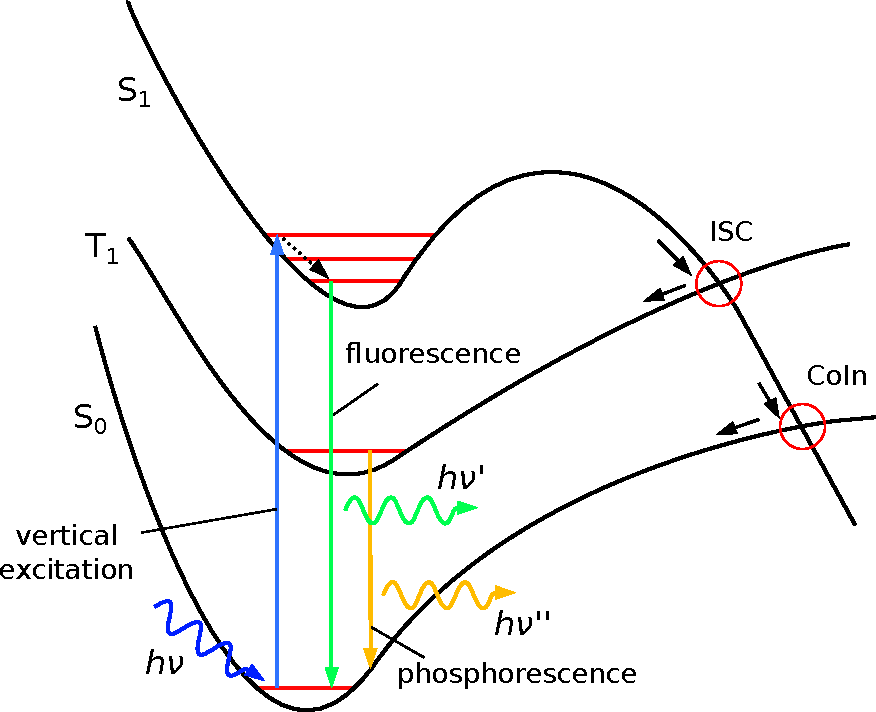
\includegraphics[scale=0.8]{Pics/PESEX}
\caption{Potential energy surface}
\label{fig:PESEX}
\end{figure}

\section{Delta Methods}

\section{The Algebraic Diagrammatic Construction Method}

\section{Response Theory}

\section{Equation-of-Motion}

\section{Time-dependent stuff?}